\chapter{\texorpdfstring{\codeplain{pdmat}}{pdmat}: Known Parameter-Dependent Matrices}
\label{sec:pdmat}

\code{pdmat} stores known finite real matrix data on a tensor grid. Objects can be coefficient-backed, function-only, or function-backed with explicit Bernstein coefficient evidence. Coefficient-backed objects participate in algebra. Function-only objects evaluate exactly through the stored handle and reserve \code{bernTable} and coefficient algebra for objects with coefficient evidence. Shared matrix-shape, unary, structural, reduction, reordering, and repetition methods are implemented centrally by \code{pdbase} and remain complete public \code{pdmat} behavior. This chapter documents their known-data syntax, numeric examples, validations, and boundaries.

For coefficient-backed data, one storage cell is the pullback $A^{(\vect{c})}=A\circ\phi_{\vect{c}}$, with local expansion
\begin{gather}
    \label{eq:bernstein-coeffs}
    A^{(\vect{c})}(\vect{\alpha})=\displaystyle\sum_{\vect{i}\in\prod_{s=1}^{\ell}\{0,\ldots,m_s\}}B_{\vect{i}}^{\vect{m}}(\vect{\alpha})A^{(\vect{c})}[\vect{i}]
\end{gather}
with $\vect{\alpha}=\phi_{\vect{c}}^{-1}(\vect{\rho})$. Construction chooses the source of those coefficients. \code{evaluate} reconstructs the matrix value. \code{elevate} changes the coefficient representation while preserving the polynomial. Matrix multiplication applies the binomial-weighted convolution, with details given in \cref{sec:bernstein-product-math}. A function-backed object keeps exact handle evaluation separate from its finite coefficient evidence, while a function-only object supports exact evaluation exclusively.

The chapter follows these three source families. A global or nested coefficient source supports coefficient inspection and algebra, a function with an explicit degree retains both exact evaluation and validated coefficient evidence, and a function constructed with the degree omitted supports exact evaluation only. The examples therefore inspect the source state before using elevation, plotting, algebra, or comparison.

\section{API Map}
\label{sec:pdmat-lookup}

\begin{tabularx}{\textwidth}{@{}lY@{}}
\toprule
Task & Entry \\
\midrule
Construct data &
\hyperref[sec:pdmat-construction]{\codeplain{pdmat}} \\
Public properties &
\hyperref[sec:pdmat-properties]{\codeplain{GridInfo}/\codeplain{MatrixSize}/\codeplain{Degree}/\codeplain{LocalValues} and metadata} \\
Inspect backend storage &
\hyperref[sec:pdmat-backend-inheritance]{\codeplain{cells}/\codeplain{lbls}/\codeplain{coeffs} and counts} \\
Evaluate &
\hyperref[sec:pdmat-evaluate]{\codeplain{evaluate}} \\
Differentiate &
\hyperref[sec:pdmat-rhodiff]{\codeplain{rhodiff}} \\
Inspect/display &
\hyperref[sec:pdmat-table]{\codeplain{bernTable}},
\hyperref[sec:pdmat-display]{\codeplain{disp}},
\hyperref[sec:pdmat-display]{\codeplain{display}} \\
Plot &
\hyperref[sec:pdmat-plot]{\codeplain{plot}} \\
Arithmetic &
\hyperref[sec:pdmat-algebra]{\codeplain{+}},
\hyperref[sec:pdmat-algebra]{\codeplain{-}},
\hyperref[sec:pdmat-algebra]{unary \codeplain{+}/\codeplain{-}},
\hyperref[sec:pdmat-algebra]{\codeplain{*}} \\
Compare/certify &
\hyperref[sec:pdmat-comparison]{logical \codeplain{==} and known-data \codeplain{<=}/\codeplain{>=}} \\
Matrix methods &
\hyperref[sec:pdmat-matrix-ops]{shape and structural methods} \\
Elevate Bernstein storage &
\hyperref[sec:pdmat-elevate]{\codeplain{elevate}} \\
Index/assign entries &
\hyperref[sec:pdmat-indexing]{indexing and assignment} \\
\bottomrule
\end{tabularx}

\section{Construct \texorpdfstring{\codeplain{pdmat}}{pdmat} Objects}
\label{sec:pdmat-construction}

\syntaxhead
\begin{lstlisting}[style=dpsyntax]
A = pdmat(gridVector, source)
A = pdmat(gridVector, source, Degree=degree)
A = pdmat(gridVector, source, RateBounds=rb)
A = pdmat(gridVectors, source)
A = pdmat(gridVectors, source, Degree=degree, RateBounds=rb)
A = pdmat(..., ValidationMode=mode)
\end{lstlisting}

\arghead
\begin{itemize}[leftmargin=*]
  \item \code{gridVector} is a numeric vector used as a one-parameter grid shorthand, such as \code{[0 1 2]}.
  \item \code{gridVectors} is a cell vector with one numeric grid vector per parameter, such as \code{{[0 1], [10 20]}}.
  \item \code{source} may be:
  \begin{enumerate}
      \item A function handle, e.g., \code{@(rho) [rho rho^2]} is a one-parameter $2\times 1$ matrix function
      \item A global cell grid of numeric Bernstein coefficients, e.g., \code{{[1 2], [3 4]}} is a two-cell degree-one grid with two $1\times1$ coefficients per cell.
      \item A explicit nested \code{LocalValues}, e.g., \code{{1, 2, 3}} is scalar degree-two data on one cell.
  \end{enumerate}
  \item \code{Degree=degree} accepts one finite nonnegative integer scalar shorthand or an $\ell$-element vector and is stored as a $1$-by-$\ell$ row $\vect{m}=(m_1,\ldots,m_\ell)$. A scalar expands uniformly. An explicitly supplied scalar on a multidimensional grid emits \codeerr{pdmat}{ScalarDegreeExpansion} once. Omitted degree inference, function-only defaults, and one-dimensional forms remain warning-free. For function handles, omitting \code{Degree} creates a function-only object. Supplying \code{Degree} validates and stores Bernstein coefficient evidence while retaining the exact function handle for \code{evaluate}.
  \item \code{RateBounds=rb} is an $\ell$-by-$2$ finite real matrix of lower and upper scheduling-rate bounds and is accepted with every source family. With an ordinary one-row source it is metadata used by \code{rhodiff}. An explicit nested leaf may instead contain either one ordinary row or all $N_v=\code{size(helper.rateVerts(rb),1)}$ distinct-vertex rows, uniformly across every physical cell, in \code{helper.rateVerts(rb)} order. A fixed rate direction contributes one value, so $N_v\le 2^\ell$.
  \item \code{ValidationMode=mode} accepts scalar text \code{"fast"} or \code{"strict"}, case-insensitively, and defaults to \code{"fast"}. It controls only repeated post-normalization structural checks and remains transient call state. Public source validation remains complete in both modes.
\end{itemize}

Both \code{pdmat} and \code{pdvar} constructors share the same normalization expression as in \cref{eq:bernstein-coeffs}, which inherited from \code{pdbase}. A \code{pdmat} validates known source data, while a \code{pdvar} creates and shares YALMIP control matrices. The basis and storage mathematics are given in \cref{sec:bernstein-tensor-grids}.

\begin{figure}[H]
\centering
\begin{tikzpicture}[node distance=7mm and 7mm,
  choice/.style={dp/call-branch,diamond,aspect=2,text width=15mm,
    minimum height=9mm,inner sep=1pt}]
  \node[dp/call-entry] (entry) {\hyperref[sec:pdmat-construction]{\codeplain{pdmat}} or\\\hyperref[sec:pdvar-construction]{\codeplain{pdvar}}};
  \node[dp/call-step,right=of entry] (parse) {parse dimensions, source,\\and options};
  \node[dp/call-step,right=of parse] (normal) {\code{mkGrid} and \code{normDeg}\\normalize $\mathcal G$ and $\vect{m}$};
  \node[choice,below=of normal] (fork) {constructor\\kind};
  \node[dp/call-branch,below left=9mm and 18mm of fork] (source) {\code{pdmat}: source conversion\\or function validation};
  \node[dp/call-branch,below right=9mm and 18mm of fork] (control) {\code{pdvar}: control lattice\\and shared-face handles};
  \node[dp/call-result,below=25mm of fork] (store) {\hyperref[sec:pdbase-constructor]{\codeplain{pdbase}}\\cell-wise storage};
  \draw[dp/call-arrow] (entry) -- (parse);
  \draw[dp/call-arrow] (parse) -- (normal);
  \draw[dp/call-arrow] (normal) -- (fork);
  \draw[dp/call-arrow] (fork) -- (source);
  \draw[dp/call-arrow] (fork) -- (control);
  \draw[dp/call-arrow] (source) -- (store.west);
  \draw[dp/call-arrow] (control) -- (store.east);
\end{tikzpicture}
\caption{Constructor call path. The public parser chooses known-source conversion or decision-control construction after the common grid and vector-degree normalization.}
\label{fig:constructor-call-path}
\end{figure}

\examplehead
The scalar-grid shorthand is the shortest coefficient-backed form.  The three numeric cells below are the global Bernstein coefficients for two physical cells with degree one.

\begin{lstlisting}[style=dpmatlab]
A = pdmat([0 1 2], {10, 20, 30}, Degree=1);
disp(A)
matrixSize = size(A)
degree = A.Degree
sourceSummary = A.SourceSummary
\end{lstlisting}

\begin{lstlisting}[style=dpoutput]
pdmat [1 1] over 1-D grid, degree 1, source coefficient-backed, rate rows false

matrixSize = 1×2 double
     1     1

degree = 1
sourceSummary = "coefficient-backed"
\end{lstlisting}

For tensor grids, pass one grid vector per parameter. This independent example uses $\vect{m}=(2,1)$, so the first parameter has quadratic Bernstein basis and the second has linear basis. The selected-cell \code{oneLine} table prints the represented expression directly.

\begin{lstlisting}[style=dpmatlab]
B = pdmat({[0 1], [0 1]}, ...
    @(rho1, rho2) rho1.^2 + 2*rho2, Degree=[2 1]);
T = bernTable(B, [1 1], "oneLine");
disp(T)
\end{lstlisting}

\begin{lstlisting}[style=dpoutput]
    CellSubscript
    _____________

       {[1 1]}
\end{lstlisting}
\begin{lstlisting}[style=dpwideoutput]
    Expression
    _________________________________________________________________________________________________________________

    "(1-α1)^2 * (1-α2)*0 + (1-α1)^2 * α2*2 + 2(1-α1)α1 * (1-α2)*0 + 2(1-α1)α1 * α2*2 + α1^2 * (1-α2)*1 + α1^2 * α2*3"
\end{lstlisting}

Use explicit nested \code{LocalValues} when each physical cell must be written directly.  Here each cell stores two $1\times2$ row-vector coefficients.

\begin{lstlisting}[style=dpmatlab]
localVals = {{[1 0], [0 1]}, {[0 1], [0 2]}};
C = pdmat({[0 1 2]}, localVals, Degree=1);
disp(C)
matrixSize = size(C)
secondCellCoefficients = cell2mat(C.coeffs(2))
\end{lstlisting}

\begin{lstlisting}[style=dpoutput]
pdmat [1 2] over 1-D grid, degree 1, source coefficient-backed, rate rows false

matrixSize = 1×2 double
     1     2

secondCellCoefficients = 1×4 double
     0     1     0     2
\end{lstlisting}

When \code{source} is a function handle and \code{Degree} is omitted, the object stores the exact evaluator exclusively.

\begin{lstlisting}[style=dpmatlab]
F = pdmat({[0 1]}, @(rho) [rho rho^2]);
disp(F)
sourceSummary = F.SourceSummary
evaluatedValue = F.evaluate(0.5)
\end{lstlisting}

\begin{lstlisting}[style=dpoutput]
pdmat [1 2] over 1-D grid, degree 1, source function, rate rows false

sourceSummary = "function"
evaluatedValue = 1×2 double
    0.5000    0.2500
\end{lstlisting}

Add \code{Degree} for a polynomial function when later coefficient inspection or algebra should use Bernstein evidence.  The exact function handle is still used for point evaluation.

\begin{lstlisting}[style=dpmatlab]
G = pdmat({[0 1]}, @(rho) rho.^2, Degree=2);
disp(G)
sourceSummary = G.SourceSummary
firstCellCoefficients = cell2mat(G.coeffs(1))
\end{lstlisting}

\begin{lstlisting}[style=dpoutput]
pdmat [1 1] over 1-D grid, degree 2, source function-bernstein, rate rows false

sourceSummary = "function-bernstein"
firstCellCoefficients = 1×3 double
     0     0     1
\end{lstlisting}

These forms all create finite known-data objects, but only the coefficient- backed and function-Bernstein forms can participate in coefficient algebra.

\remarkshead
\code{FunctionHandle} retains the supplied function handle for function-only and function-Bernstein sources. It is empty for cell-backed sources. Its set access is private.
\begin{itemize}[leftmargin=*]
  \item Constructor option errors use \codeerr{pdmat}{InvalidOptions}, \codeerr{pdmat}{Unsupported}\allowbreak\code{Option}, or \codeerr{pdmat}{Unknown}\allowbreak\code{Option}. Grid errors use \codeerr{pdmat}{InvalidGrid} or \codeerr{pdmat}{Invalid}\allowbreak\code{GridVector}.
  \item Source and function validation uses \codeerr{pdmat}{InvalidSource}, \codeerr{pdmat}{Invalid}\allowbreak\code{FunctionHandle}, \codeerr{pdmat}{Invalid}\allowbreak\code{FunctionOutput}, or \codeerr{pdmat}{InvalidData}.
  \item Degree, rate, and storage failures use \codeerr{pdmat}{InvalidDegree}, \codeerr{pdmat}{Invalid}\allowbreak\code{RateBounds}, \codeerr{pdmat}{Invalid}\allowbreak\code{Local}\allowbreak\code{Values}, \codeerr{pdmat}{Invalid}\allowbreak\code{Coefficient}\allowbreak\code{Cell}, or \codeerr{pdmat}{Invalid}\allowbreak\code{Coefficient}\allowbreak\code{Payload}. Explicit multidimensional scalar degree expansion is accepted with warning \codeerr{pdmat}{ScalarDegreeExpansion}.
  \item Invalid validation modes raise \codeerr{pdmat}{Invalid}\allowbreak\code{ValidationMode}. With explicit \code{Degree}, nonrepresentable functions raise \codeerr{pdmat}{NonBernstein}\allowbreak\code{Polynomial}. Invalid validation probes raise \codeerr{pdmat}{Invalid}\allowbreak\code{FunctionValue}.
  \item Mismatched shared faces are retained as discontinuous local data and emit warning \codeerr{pdmat}{Discontinuous}\allowbreak\code{LocalValues}.
\end{itemize}

\section{Public Properties}\index{GridInfo@\texttt{GridInfo}}\index{MatrixSize@\texttt{MatrixSize}}\index{Degree@\texttt{Degree}}\index{LocalValues@\texttt{LocalValues}}\index{IsContinuous@\texttt{IsContinuous}}\index{ContainsDecision@\texttt{ContainsDecision}}\index{NumRateRows@\texttt{NumRateRows}}\index{RateBounds@\texttt{RateBounds}}\index{SourceSummary@\texttt{SourceSummary}}\index{FunctionHandle@\texttt{FunctionHandle}}
\label{sec:pdmat-properties}

Every \code{pdmat} property is public and read-only with private set access. Dot access exposes the known-data representation, while constructors and algebra return new values when stored information changes.

\begin{tabularx}{\textwidth}{@{}p{0.20\textwidth}Y@{}}
\toprule
Property & Stored information \\
\midrule
\code{GridInfo} & A scalar tensor-grid structure. \code{Vectors} is a $1$-by-$\ell$ cell row of axis grids, \code{Points} is a $\prod_{s=1}^{\ell}k_s$-by-$\ell$ numeric matrix of physical grid nodes in combination order, \code{Bounds} is the $\ell$-by-$2$ parameter box, and \code{NumNodes} is the $1$-by-$\ell$ row $[k_1,\ldots,k_\ell]$. \\
\code{MatrixSize} & The two-element row $[n_r,n_c]$ giving the size of every known matrix coefficient and every evaluated matrix. \\
\code{Degree} & The $1$-by-$\ell$ row $[m_1,\ldots,m_\ell]$ of local Bernstein degrees used in every physical cell. \\
\code{LocalValues} & The $\ell$-level nested physical-cell tree with $k_s-1$ cells along direction $s$. Each ordinary leaf is a $1$-by-$\prod_{s=1}^{\ell}(m_s+1)$ cell row of finite real numeric matrices in \code{lbls(A)} order. An explicit-rate leaf is \code{NumRateRows}-by-$\prod_{s=1}^{\ell}(m_s+1)$ in stored rate-vertex order. Function-only objects contain placeholder storage that provides zero Bernstein coefficient evidence. \\
\code{IsContinuous} & A logical scalar recording whether adjacent coefficient-backed cells match on shared faces. Function-backed data with verified Bernstein evidence are continuous, while accepted mismatched nested local values set this flag false. \\
\code{ContainsDecision} & Always false for \code{pdmat}, because its stored coefficient payloads are known numeric data. \\
\code{NumRateRows} & A nonnegative integer scalar giving the number of explicit rate-vertex rows in each leaf. Zero denotes ordinary one-row storage even when \code{RateBounds} is present only as metadata. \\
\code{RateBounds} & Empty or an $\ell$-by-$2$ matrix whose row $s$ gives the lower and upper bounds for $\dot{\rho}_s$. Distinct rate vertices use the package-wide lower-then-upper combination order. \\
\code{SourceSummary} & Scalar origin text such as \code{"coefficient-backed"}, \code{"function"}, \code{"function-bernstein"}, or \code{"derivative"}. \\
\code{FunctionHandle} & The supplied function handle for function-only and function-Bernstein sources. It is empty for cell-backed sources and for numeric results whose construction clears exact function state. \\
\bottomrule
\end{tabularx}

\examplehead
\begin{lstlisting}[style=dpmatlab]
A = pdmat({[0 1]}, @(rho) [rho.^2, 1+rho], ...
    Degree=2, RateBounds=[-1 1]);
gridBounds = A.GridInfo.Bounds
nodeCounts = A.GridInfo.NumNodes
matrixSize = A.MatrixSize
degree = A.Degree
firstLeafSize = size(A.LocalValues{1})
isContinuous = A.IsContinuous
containsDecision = A.ContainsDecision
rateRowCount = A.NumRateRows
rateBounds = A.RateBounds
sourceSummary = A.SourceSummary
hasFunction = ~isempty(A.FunctionHandle)
\end{lstlisting}
\begin{lstlisting}[style=dpoutput]
gridBounds = 1×2 double
     0     1
nodeCounts = 2
matrixSize = 1×2 double
     1     2
degree = 2
firstLeafSize = 1×2 double
     1     3
isContinuous =
  logical
   1
containsDecision =
  logical
   0
rateRowCount = 0
rateBounds = 1×2 double
    -1     1
sourceSummary = "function-bernstein"
hasFunction =
  logical
   1
\end{lstlisting}

Direct assignments such as \code{A.Degree = 1} or \code{A.FunctionHandle = []} raise MATLAB's private-set property error. Construct a new \code{pdmat}, or use a public operation that returns one, to change the represented value.

\paragraph{Related APIs.}
Use \cref{sec:pdmat-backend-inheritance} to traverse \code{LocalValues}, \cref{sec:pdmat-evaluate} to reconstruct a matrix, and \cref{sec:pdbase-fields} for the backend implementation contract.


\section{Inspect Inherited Bernstein Storage}\index{cells@\texttt{cells}}\index{lbls@\texttt{lbls}}\index{coeffs@\texttt{coeffs}}\index{ncell@\texttt{ncell}}\index{ncoeff@\texttt{ncoeff}}\index{npar@\texttt{npar}}
\label{sec:pdmat-backend-inheritance}

\syntaxhead
\begin{lstlisting}[style=dpsyntax]
cellSubs = cells(A)
cellSubs = A.cells()
labels = lbls(A)
labels = A.lbls()
coefficients = coeffs(A, cellSubs)
coefficients = A.coeffs(cellSubs)
n = ncell(A)
n = A.ncell()
n = ncoeff(A)
n = A.ncoeff()
n = npar(A)
n = A.npar()
\end{lstlisting}

\descriptionhead
The inherited implementation follows the shared \code{pdbase} traversal order. \code{cells} returns an \code{ncell(A)}-by-$\ell$ numeric matrix with one physical-cell subscript per row and component $c_s\in\left\{1,\ldots,k_s-1\right\}$, where $k_s=\code{A.GridInfo.NumNodes}(s)$. \code{lbls} returns an \code{ncoeff(A)}-by-$\ell$ numeric matrix of tensor labels with component $i_s\in\left\{0,\ldots,m_s\right\}$. Both use the package-wide combination order. \code{coeffs} returns the selected flat leaf in that label order: an ordinary known-data leaf is a $1$-by-\code{ncoeff(A)} cell row of numeric matrices, while an explicit-rate leaf is \code{A.NumRateRows}-by-\code{ncoeff(A)} in stored rate-vertex order.

The counts are \code{ncell(A)}$=\prod_{s=1}^{\ell}(\code{A.GridInfo.NumNodes}(s)-1)$, \code{ncoeff(A)}$=\prod_{s=1}^{\ell}(\code{A.Degree}(s)+1)$, and \code{npar(A)}$=\ell=\code{numel(A.GridInfo.Vectors)}$. Function-only data still expose their grid, labels, counts, and placeholder leaf. Coefficient-dependent operations such as \code{bernTable}, elevation, and algebra require actual coefficient evidence.

\examplehead
\begin{lstlisting}[style=dpmatlab]
A = pdmat({[0 1]}, {1, 2}, Degree=1);
physicalCells = A.cells()
labels = A.lbls()
sourceCoefficients = cell2mat(A.coeffs(1))
counts = [A.ncell(), A.ncoeff(), A.npar()]
\end{lstlisting}
\begin{lstlisting}[style=dpoutput]
physicalCells = 1
labels = 2×1 double
     0
     1
sourceCoefficients = 1×2 double
     1     2
counts = 1×3 double
     1     2     1
\end{lstlisting}

\remarkshead
Invalid physical-cell selectors raise \codeerr{pdbase}{InvalidCellSubs}.

\paragraph{Related APIs.}
Use \cref{sec:pdmat-properties} for the stored tree and metadata, \cref{sec:pdmat-table} for formatted coefficient inspection, and \cref{sec:pdbase-inspection,sec:pdbase-counts} for the backend implementation details.

\section{\texorpdfstring{\codeplain{evaluate}}{evaluate}}
\index{evaluate@\texttt{evaluate}}
\label{sec:pdmat-evaluate}

\syntaxhead
\begin{lstlisting}[style=dpsyntax]
val = evaluate(A, point)
val = A.evaluate(point)
\end{lstlisting}

\arghead
\begin{itemize}[leftmargin=*]
  \item \code{A} is a \code{pdmat} object. \item \code{point} is a finite real scalar for a one-parameter object, such as \code{0.25}, or a finite real row vector with one entry per parameter, such as \code{[0.25 12]}.  Every entry must lie within the corresponding grid bounds. \item \code{val} is a numeric matrix with \code{size(A)}.  Coefficient-backed objects use local Bernstein interpolation. Function-backed objects call their stored function handle.
\end{itemize}

\remarkshead
A point with the wrong type, length, or finite-real shape raises \codeerr{pdmat}{InvalidPoint}. A point outside any grid bound raises \codeerr{pdmat}{PointOutOfBounds}.  If a stored function fails or returns a nonfinite, complex, empty, or size-inconsistent matrix at the requested point, \code{evaluate} raises \codeerr{pdmat}{Invalid}\allowbreak\code{FunctionValue}.

For a degree-one scalar coefficient-backed object on $[\rho_1^{(1)},\rho_1^{(2)}]$,
\begin{gather*}
A(\rho) = (1-\alpha)A^{(c)}[0]+\alpha A^{(c)}[1],\qquad
  \alpha = \frac{\rho_1-\rho_1^{(1)}}
                 {\rho_1^{(2)}-\rho_1^{(1)}}.
\end{gather*}
The same local-coordinate rule is applied entrywise for matrix-valued data.

\begin{center}
\begin{tikzpicture}[x=5.4cm,y=0.72cm]
  \draw[->,black!65] (0,0)--(1.08,0) node[right,font=\scriptsize] {$\rho$};
  \draw[->,black!65] (0,0)--(0,4.35) node[above,font=\scriptsize] {$A(\rho)$};
  \draw[very thick,dpblue,domain=0:1,samples=70,smooth]
    plot (\x,{2+6*\x-5*\x*\x});
  \filldraw[fill=white,draw=black!70] (0,2) circle (1.5pt);
  \node[above=3pt,anchor=east,font=\scriptsize] at (-0.03,2)
  {$A^{(c)}[0]=2$};
  \foreach \x/\y/\lab in {0.5/3.75/{A^{(c)}[1]=5},1/3/{A^{(c)}[2]=3}}{
    \filldraw[fill=white,draw=black!70] (\x,\y) circle (1.5pt);
    \node[above=3pt,font=\scriptsize] at (\x,\y) {$\lab$};}
  \def\evalx{0.35}
  \def\evaly{3.4875}
  \draw[densely dashed,black!60] (\evalx,0)--(\evalx,\evaly);
  \filldraw[fill=dpblue,draw=dpblue] (\evalx,\evaly) circle (1.7pt);
  \node[below=3pt,font=\scriptsize] at (\evalx,0)
    {$\rho_\star$};
  \node[dp/label,anchor=west] at (0.39,2.65)
    {$\code{Astar=A.evaluate(rhoStar)}$};
\end{tikzpicture}

\textit{Evaluation follows the degree-two Bernstein curve with coefficients $[2,5,3]$. The dashed line locates the requested physical point.}
\end{center}

\examplehead
Use the function-call form when the object is naturally one input among several MATLAB expressions.

\begin{lstlisting}[style=dpmatlab]
A = pdmat({[0 1]}, {2, 4}, Degree=1);
val = evaluate(A, 0.25)
\end{lstlisting}

\begin{lstlisting}[style=dpoutput]
val = 2.5000
\end{lstlisting}

At $\rho=0.25$, the public local coordinate is $\alpha=0.25$, so the interpolated value is $0.75\cdot2+0.25\cdot4=2.5$.

The dot-call form is equivalent and can be convenient in command-window exploration.

\begin{lstlisting}[style=dpmatlab]
A = pdmat({[0 1]}, {2, 4}, Degree=1);
val = A.evaluate(0.75)
\end{lstlisting}

\begin{lstlisting}[style=dpoutput]
val = 3.5000
\end{lstlisting}

Function-backed objects route through the retained function handle, so non-polynomial expressions can still be evaluated exactly at a point.

\begin{lstlisting}[style=dpmatlab]
F = pdmat({[0 pi]}, @(rho) sin(rho));
val = F.evaluate(pi/2)
\end{lstlisting}

\begin{lstlisting}[style=dpoutput]
val = 1
\end{lstlisting}

\enlargethispage{3\baselineskip}
\section{Differentiate Known Data with \texorpdfstring{\codeplain{rhodiff}}{rhodiff}}
\index{rhodiff@\texttt{rhodiff}}\index{rate row}
\label{sec:pdmat-rhodiff}

\syntaxhead
\begin{lstlisting}[style=dpsyntax]
D = rhodiff(A)
D = rhodiff(A, rateBounds)
\end{lstlisting}

\arghead \code{rhodiff} differentiates coefficient-backed \code{pdmat} data cell by cell and returns a \code{pdmat} with numeric rate-vertex rows. Explicit \code{rateBounds} supplies missing metadata, and when \code{A.RateBounds} is already stored, the explicit bounds must match it exactly. Empty bounds from both sources raise \codeerr{pdmat}{MissingRateBounds}. Along axis $s$, the local derivative coefficients are $\frac{m_s}{h_s^{\vect{c}}}\bigl(A^{(\vect{c})}[\vect{i}+\vect{e}_s]-A^{(\vect{c})}[\vect{i}]\bigr)$. For one parameter, the input degree is still the vector $\vect{m}=(m_1)$. If $m_1>0$, the result degree is $(m_1-1)$, while $\vect{m}=(0)$ remains $(0)$. For more than one parameter, each nonzero-axis partial is elevated exactly from $\vect{m}-\vect{e}_s$ back to the common tensor degree $\vect{m}=\code{A.Degree}$ before summation. A zero-degree axis contributes zero, and an all-zero tensor degree produces complete zero rate rows. The result is rate-dependent and generally discontinuous across cell faces. \Cref{sec:bernstein-differentiation,sec:bernstein-rate-vertex-storage} derive the reduction, re-elevation, and deterministic rate-row order. A function-only source raises \codeerr{pdmat}{FunctionOnlyDiff}. Malformed or inconsistent bounds raise \codeerr{pdmat}{InvalidRateBounds} or \codeerr{pdmat}{RateBoundsMismatch}, and data that already contain explicit rate rows, including a previous derivative, raise \codeerr{pdmat}{InvalidDiff}.

The implementation constructs the distinct rate vertices first. It then forms each cell partial, re-elevates multivariate partials exactly to the common degree, combines them with each rate vertex, and returns the owning value class through its \code{mkRhodiff} method. The derivative formula and rate-row layout are given in \cref{sec:bernstein-differentiation,sec:bernstein-rate-vertex-storage}.

\begin{figure}[H]
\centering
\begin{tikzpicture}[node distance=5.5mm]
  \node[dp/call-entry] (entry) {\code{rhodiff}};
  \node[dp/call-step,right=of entry] (verts) {\code{rateVerts}};
  \node[dp/call-step,right=of verts] (partial) {cell partials};
  \node[dp/call-step,right=of partial] (elev) {exact\\re-elevation};
  \node[dp/call-step,right=of elev] (combine) {rate-weighted\\combination};
  \node[dp/call-result,below=of elev] (result) {class-specific\\\code{mkRhodiff}};
  \draw[dp/call-arrow] (entry) -- (verts);
  \draw[dp/call-arrow] (verts) -- (partial);
  \draw[dp/call-arrow] (partial) -- (elev);
  \draw[dp/call-arrow] (elev) -- (combine);
  \draw[dp/call-arrow] (combine.south) |- (result.east);
\end{tikzpicture}
\caption{Differentiation call path. Cell partials are combined only after their tensor degrees and the rate-vertex order are fixed.}
\label{fig:rhodiff-call-path}
\end{figure}

\examplehead
\begin{lstlisting}[style=dpmatlab]
A = pdmat([0 1], {0, 2}, Degree=1, RateBounds=[-1 2]);
D = rhodiff(A);
T = bernTable(D, 1, "oneLine");
disp(T)
\end{lstlisting}

\begin{lstlisting}[style=dpoutput]
    CellSubscript    RateVertexIndex    RateVertex    Expression
    _____________    _______________    __________    __________

        {[1]}               1              {[-1]}       "1*-2"
        {[1]}               2              {[ 2]}       "1*4"
\end{lstlisting}

In several parameters, each partial is restored to the common tensor degree before the rate-weighted sum. Here the four rate rows are constant over all four local labels, but the stored degree remains $[1,1]$.

\begin{lstlisting}[style=dpmatlab]
A = pdmat({[0 1], [0 1]}, ...
    @(rho1, rho2) rho1 + 2*rho2, ...
    Degree=[1 1], RateBounds=[-1 1; -2 3]);
D = rhodiff(A);
T = bernTable(D, [1 1], "oneLine");
disp(T)
\end{lstlisting}

\begin{lstlisting}[style=dpwideoutput]
    CellSubscript    RateVertexIndex    RateVertex                                                          Expression
    _____________    _______________    __________    _______________________________________________________________________________________________________________________

       {[1 1]}              1           {[-1 -2]}     "(1-α1)^2 * (1-α2)*-4 + (1-α1)^2 * α2*-4 + 2(1-α1)α1 * (1-α2)*-5 + 2(1-α1)α1 * α2*-5 + α1^2 * (1-α2)*-6 + α1^2 * α2*-6"
       {[1 1]}              2           {[ -1 3]}     "(1-α1)^2 * (1-α2)*6 + (1-α1)^2 * α2*6 + 2(1-α1)α1 * (1-α2)*5 + 2(1-α1)α1 * α2*5 + α1^2 * (1-α2)*4 + α1^2 * α2*4"
       {[1 1]}              3           {[ 1 -2]}     "(1-α1)^2 * (1-α2)*-4 + (1-α1)^2 * α2*-4 + 2(1-α1)α1 * (1-α2)*-3 + 2(1-α1)α1 * α2*-3 + α1^2 * (1-α2)*-2 + α1^2 * α2*-2"
       {[1 1]}              4           {[  1 3]}     "(1-α1)^2 * (1-α2)*6 + (1-α1)^2 * α2*6 + 2(1-α1)α1 * (1-α2)*7 + 2(1-α1)α1 * α2*7 + α1^2 * (1-α2)*8 + α1^2 * α2*8"
\end{lstlisting}

\section{Inspect Coefficients and Plot Values}
\label{sec:pdmat-visualization}

\subsection{\texorpdfstring{\codeplain{bernTable}}{bernTable}}
\index{bernTable@\texttt{bernTable}}
\label{sec:pdmat-table}

\syntaxhead
\begin{lstlisting}[style=dpsyntax]
T = bernTable(A)
T = bernTable(A, cellSubs)
T = bernTable(A, "oneLine")
T = bernTable(A, cellSubs, "oneLine")
\end{lstlisting}

\arghead
\begin{itemize}[leftmargin=*]
  \item \code{cellSubs} selects one physical cell. \item \code{"oneLine"} returns one row per selected physical cell and rate vertex with a compact Bernstein expression. \item The detailed default form uses seven metadata columns. An explicit-rate-row object additionally includes \code{RateVertexIndex} and \code{RateVertex}. Their deterministic distinct-vertex order is \code{helper.rateVerts(A.RateBounds)} order.
\end{itemize}

For one parameter, write the stored degree vector as $\vect{m}=(m_1)$. The \code{Basis} column reports
\begin{gather*}
  \binom{m_1}{j}(1-\alpha)^{m_1-j}\alpha^j.
\end{gather*}
For multiple parameters, the basis is the tensor product of that expression in each local coordinate, using \code{alpha1}, \code{alpha2}, and so on. \code{LocalIndex} is the local Bernstein label. \code{CoeffSubscript} maps the local label back to the global coefficient subscript on the physical grid.  \code{IsPhysicalNode} is true when that coefficient lies on a physical grid node.

\begin{center}
\begin{tikzpicture}[>=Latex,node distance=7mm and 9mm,
  box/.style={dp/neutral,font=\scriptsize,
    align=center,minimum width=31mm,minimum height=10mm},
  result/.style={dp/result,
    font=\scriptsize,align=center,minimum width=36mm,minimum height=10mm}]
  \node[box] (cell) {physical cell selector\\\code{cellSubs}};
  \node[box,below=of cell] (labels) {local labels\\\code{lbls(A)}};
  \node[result,right=of cell,yshift=-7mm] (table) {\code{bernTable}\\
    cell + label + basis + value};
  \draw[->,thick,dpblue] (cell.east) -- (table.west);
  \draw[->,thick,dpblue] (labels.east) -- (table.west);
\end{tikzpicture}

\textit{The table reports stored coefficient evidence exclusively. Function sampling and solver-constraint creation belong to \code{evaluate} and \code{pdlmi}.}
\end{center}

\examplehead
\begin{lstlisting}[style=dpmatlab]
A = pdmat({[0 0.2 1]}, {[0 1], [1 1], [1 2]}, Degree=1);
T = bernTable(A, "oneLine");
disp(T)
T1 = bernTable(A, 1, "oneLine");
disp(T1)
\end{lstlisting}

\begin{lstlisting}[style=dpoutput]
    CellSubscript              Expression
    _____________    _______________________________

        {[1]}        "(1-alpha)*[0 1] + alpha*[1 1]"
        {[2]}        "(1-alpha)*[1 1] + alpha*[1 2]"

    CellSubscript              Expression
    _____________    _______________________________

        {[1]}        "(1-alpha)*[0 1] + alpha*[1 1]"
\end{lstlisting}

Use the full table when the metadata columns are the point of the example:

\begin{lstlisting}[style=dpmatlab]
A = pdmat({[0 1]}, {1, 2, 3}, Degree=2);
T = bernTable(A);
disp(T)
\end{lstlisting}

\begin{lstlisting}[style=dpwideoutput]
    TermIndex    CellSubscript    CoeffSubscript    LocalIndex          Basis          IsPhysicalNode    Value
    _________    _____________    ______________    __________    _________________    ______________    _____

        1            {[1]}            {[1]}           {[0]}       "(1-alpha)^2"            true          {[1]}
        2            {[1]}            {[2]}           {[1]}       "2(1-alpha)alpha"        false         {[2]}
        3            {[1]}            {[3]}           {[2]}       "alpha^2"                true          {[3]}
\end{lstlisting}

\remarkshead
A function-only object stores exact handle evaluation exclusively and raises \codeerr{pdmat}{FunctionOnly}\allowbreak\code{BernsteinTable}. Unknown text options, repeated selectors, or invalid physical-cell selectors raise \codeerr{pdmat}{Invalid}\allowbreak\code{BernsteinTableInput}.

For an explicit-rate-row object, \code{bernTable(A,"oneLine")} preserves the alternatives by returning one expression for every stored vertex:

\begin{lstlisting}[style=dpmatlab]
A = pdmat([0 1], {{1, 3; 10, 14}}, ...
    Degree=1, RateBounds=[-1 2]);
T = bernTable(A, "oneLine");
disp("vertexIndices =")
disp(T.RateVertexIndex)
disp("rateVertices =")
disp(vertcat(T.RateVertex{:}))
disp("expressionCount =")
disp(height(T))
\end{lstlisting}

\begin{lstlisting}[style=dpoutput]
vertexIndices =
     1
     2

rateVertices =
    -1
     2

expressionCount =
     2
\end{lstlisting}

\subsection{\texorpdfstring{\codeplain{disp}}{disp} And \texorpdfstring{\codeplain{display}}{display}}
\index{disp@\texttt{disp}}\index{display@\texttt{display}}
\label{sec:pdmat-display}

\syntaxhead
\begin{lstlisting}[style=dpsyntax]
disp(A)
display(A)
A
\end{lstlisting}

\arghead \code{disp(A)} prints a compact one-line summary. \code{display(A)} is the command-window display used for an expression with assignment echo enabled. It prints grid, degree, coefficient, and source metadata.

\examplehead
\begin{lstlisting}[style=dpmatlab]
A = pdmat({[0 1]}, {1, 2}, Degree=1);
disp(A)
display(A)
\end{lstlisting}

\begin{lstlisting}[style=dpoutput]
pdmat [1 1] over 1-D grid, degree 1, source coefficient-backed, rate rows false
A =
  pdmat with 1-by-1 matrix values
  Parameters: 1
    rho_1: [0, 1], 2 nodes
  Degree: 1
  Physical cells: 1
  Coefficients per cell: 2
  Continuous: true
  Rate metadata: false
  Explicit rate rows: false
  Source: coefficient-backed
  Function handle: false
\end{lstlisting}

\subsection{\texorpdfstring{\codeplain{plot}}{plot}}\index{plot@\texttt{plot}}
\label{sec:pdmat-plot}

\syntaxhead
\begin{lstlisting}[style=dpsyntax]
h = plot(A)
h = plot(A, dims)
h = plot(A, SamplesPerCell=n)
h = plot(A, dims, SamplesPerCell=n)
h = plot(A, ..., RateVertex=k)
h = plot(A, ..., Name, Value)
\end{lstlisting}

\arghead
\begin{itemize}[leftmargin=*]
  \item \code{dims} is one or two parameter indices.  For one-parameter objects, the default is \code{1}. Otherwise the default is \code{[1 2]}, as in \code{plot(A, [1 2])}. \item \code{SamplesPerCell} is the package-owned sampling option.  The default is \code{15}. Use \code{SamplesPerCell=4} for a coarse diagnostic plot. \item \code{RateVertex=k} selects one one-based stored rate row in \code{helper.rateVerts(A.RateBounds)} order. Rate-row objects default to row one. Supplying this option for ordinary data or selecting beyond \code{A.NumRateRows} raises \codeerr{pdmat}{InvalidRateVertex}. \item Remaining name-value pairs pass through to MATLAB graphics.  One-dimensional plots pass them to \code{plot}. Two-dimensional plots pass them to \code{surf}. Examples include \code{LineWidth}, \code{FaceAlpha}, and \code{EdgeColor}. \item The output \code{h} is the vector of graphics handles, one entry per matrix element.
\end{itemize}

\remarkshead
An invalid parameter index, a repeated dimension, or a request for more than two plotting dimensions raises \codeerr{pdmat}{Invalid}\allowbreak\code{PlotDimensions}. Malformed plotting options or a nonpositive integer \code{SamplesPerCell} raise \codeerr{pdmat}{Invalid}\allowbreak\code{PlotOptions}. Errors from MATLAB graphics options remain MATLAB graphics errors. Every unselected parameter is fixed at its lower grid bound, \code{A.GridInfo.Bounds(:,1)}. A three-parameter object therefore produces a one- or two-dimensional slice plot.

For explicit rate rows, select the vertex as part of the plotting call:

\begin{lstlisting}[style=dpmatlab]
A = pdmat([0 1], {0, 2}, Degree=1, RateBounds=[-1 2]);
D = rhodiff(A);
plot(D, RateVertex=2, SamplesPerCell=20, LineWidth=2);
\end{lstlisting}

\examplehead
Each source listing below is the complete source used by \code{generate_plot_figures.m} for the adjacent result.

\textit{One-dimensional entries.}

\begin{lstlisting}[style=dpmatlab]
A = pdmat({[-1 1]}, @(rho) [rho, rho.^2]);
h = plot(A, SamplesPerCell=80, LineWidth=2);
set(h(1), "Color", [35 86 125]/255, "LineStyle", "-")
set(h(2), "Color", [0.25 0.25 0.25], "LineStyle", "--")
grid on
xlabel("rho")
ylabel("matrix entry")
title("One-dimensional pdmat entries")
legend(["A(1,1)", "A(1,2)"], "Location", "eastoutside")
\end{lstlisting}

\begin{figure}[H]
  \centering
  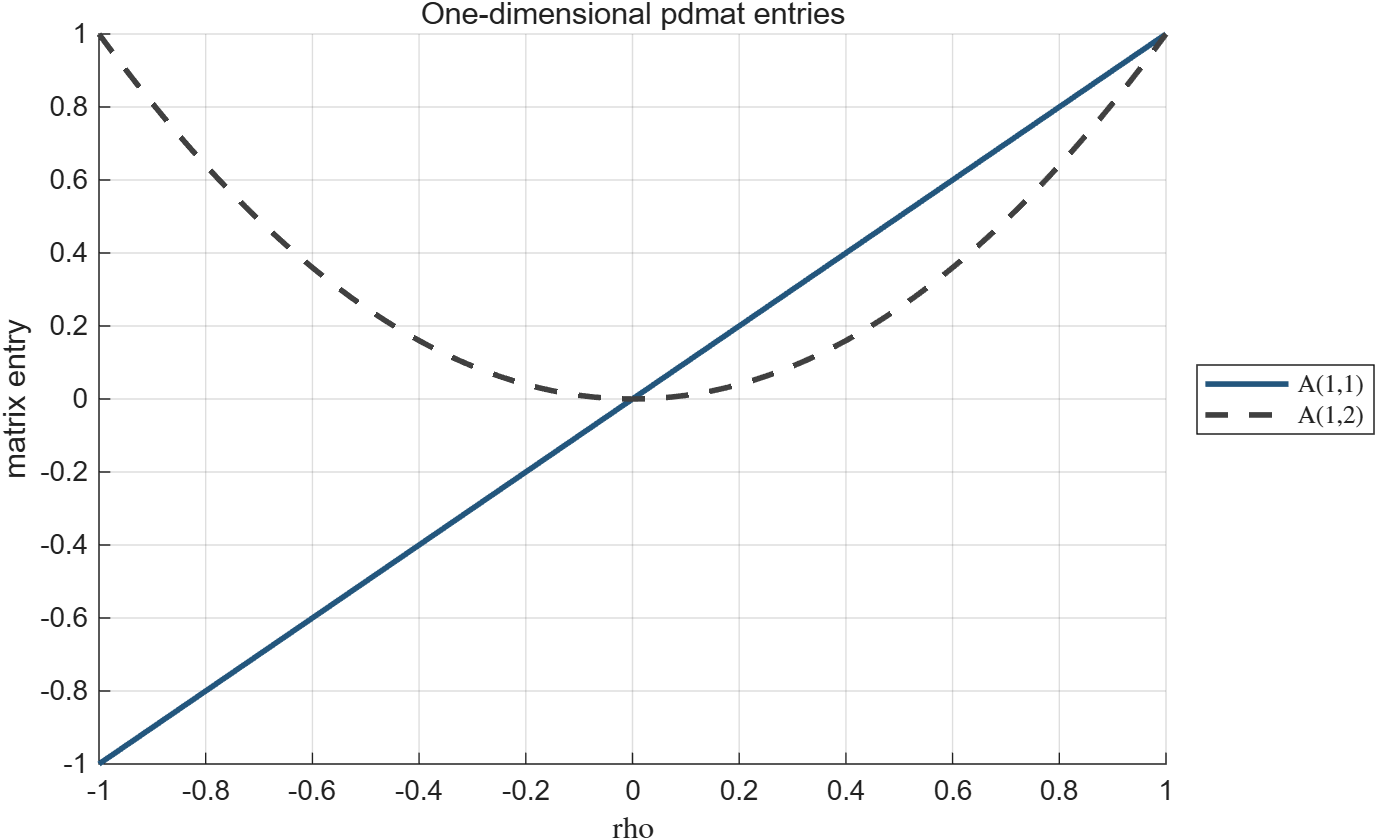
\includegraphics[width=0.65\textwidth]{matlab-figures/pdmat-plot-1d.png}
  \caption{Result of the one-dimensional source above.  The method returns one line handle per matrix entry.}
  \label{fig:pdmat-plot-1d}
\end{figure}

\textit{Two-dimensional surface.}

\begin{lstlisting}[style=dpmatlab]
A = pdmat({[-1 1], [0 2]}, ...
    @(rho1, rho2) 1 + rho1.^2 + 0.5*rho2 + rho1.*rho2);
h = plot(A, [1 2], SamplesPerCell=45, ...
    EdgeColor="none", FaceAlpha=0.78);
set(h, "FaceColor", [35 86 125]/255)
grid on
view(35, 25)
xlabel("rho1", "Interpreter", "none")
ylabel("rho2", "Interpreter", "none")
zlabel("matrix entry")
title("Two-dimensional pdmat surface")
\end{lstlisting}

\begin{figure}[H]
  \centering
  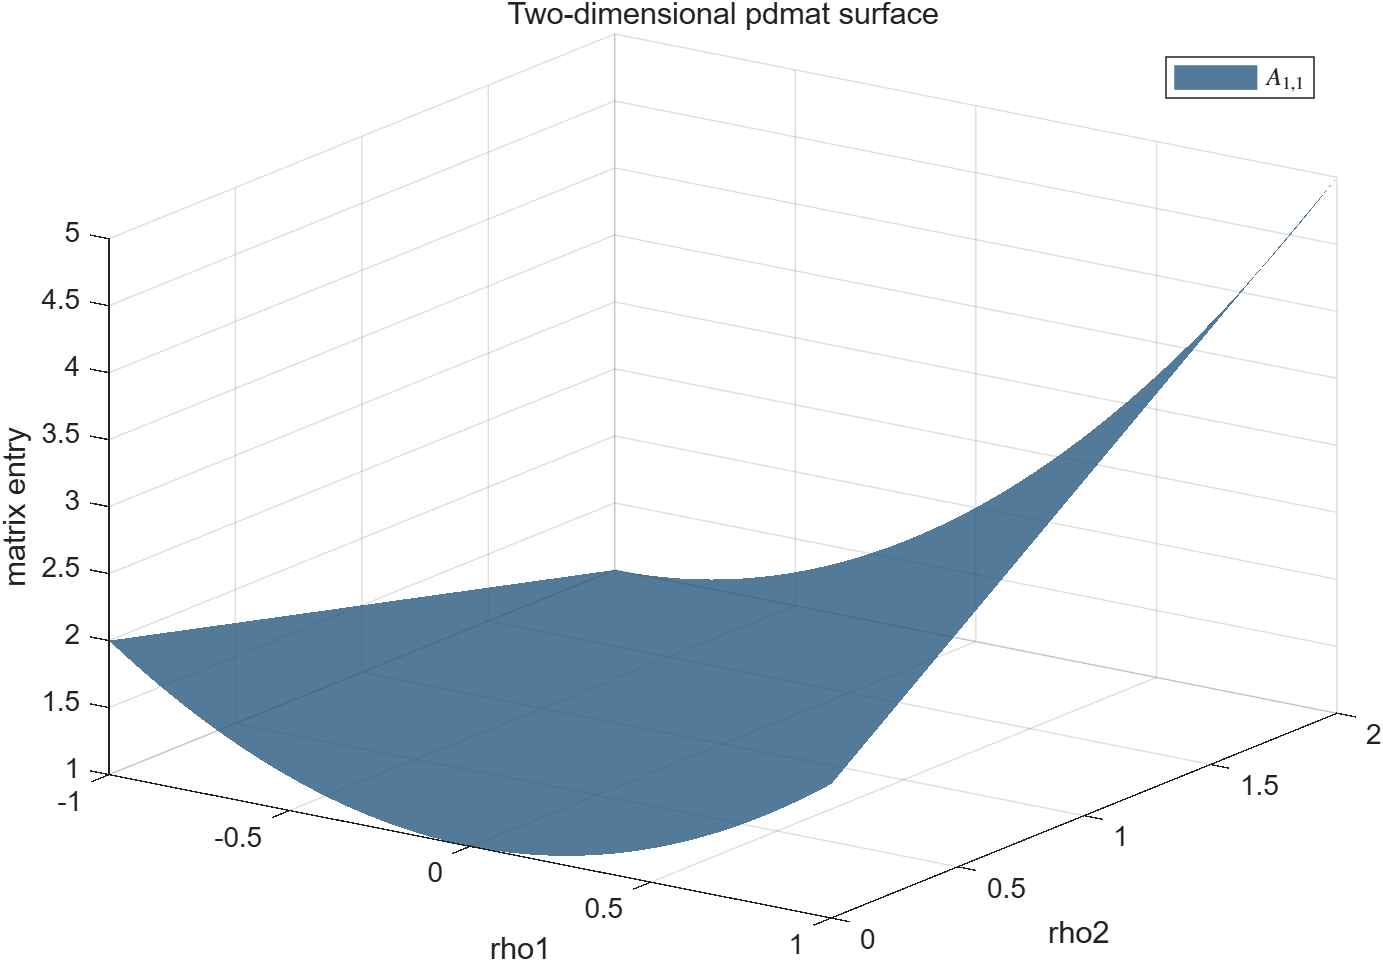
\includegraphics[width=0.65\textwidth]{matlab-figures/pdmat-plot-2d.png}
  \caption{Result of the two-dimensional source above.}
  \label{fig:pdmat-plot-2d}
\end{figure}

\textit{Two-dimensional matrix-valued surface.}

\begin{lstlisting}[style=dpmatlab]
A = pdmat({[-1 1], [0 2]}, @(rho1, rho2) [ ...
    1 + 0.8*rho1 + 0.25*rho2; ...
    1 - 0.8*rho1 + 0.25*rho2]);
h = plot(A, [1 2], SamplesPerCell=45, ...
    EdgeColor="none", FaceAlpha=0.62);
set(h(1), "FaceColor", [35 86 125]/255)
set(h(2), "FaceColor", [0.55 0.55 0.55])
grid on
view(35, 25)
xlabel("rho1", "Interpreter", "none")
ylabel("rho2", "Interpreter", "none")
zlabel("matrix entry")
title("Two entries of a 2-by-1 pdmat cross at rho1 = 0")
legend(h, ["A(1,1)", "A(2,1)"], ...
    "Location", "eastoutside")
\end{lstlisting}

The two entries are equal for every $\rho_2$ along $\rho_1=0$. Their ordering reverses on opposite sides: the first entry is lower when $\rho_1<0$ and higher when $\rho_1>0$. The crossing therefore comes from the matrix function itself.

\begin{figure}[H]
  \centering
  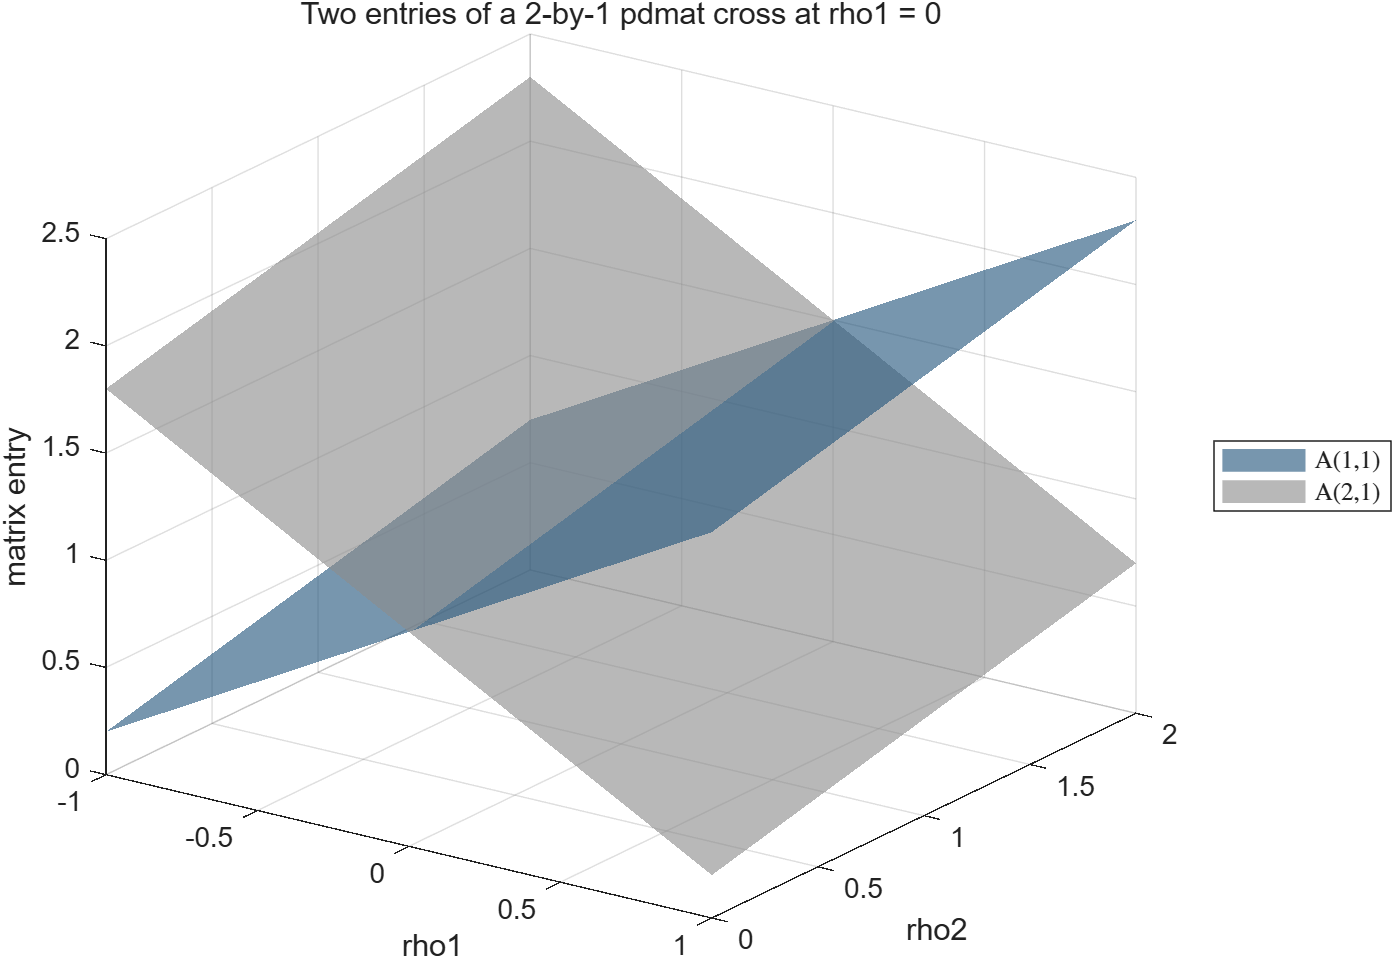
\includegraphics[width=0.65\textwidth]{matlab-figures/pdmat-plot-2d-matrix.png}
  \caption{Two entry surfaces of a $2$-by-$1$ matrix-valued function.  The outside legend distinguishes the entries while their intersection remains visible along $\rho_1=0$.}
  \label{fig:pdmat-plot-2d-matrix}
  \label{fig:pdmat-plot-3d-slice}
\end{figure}

\section{Combine Known Matrices}
\label{sec:pdmat-algebra}

A \code{pdmat} operation acts on complete matrix coefficients while the physical grid remains attached to the result.  The blocks below deliberately show one operation family at a time: purpose, supported syntax, input, immediate output, and---when the result is spatial---a before/after picture.

Addition, subtraction, concatenation, block assembly, indexing assignment, and related binary operations use the same alignment path. The path exactly refines both operands to the union grid and elevates them to the componentwise maximum degree before it assembles the requested coefficient rows. The grid and elevation mathematics are given in \cref{sec:pdbase-mergegrid,sec:bernstein-degree-elevation}.

\begin{figure}[H]
\centering
\begin{tikzpicture}[node distance=6mm]
  \node[dp/call-entry] (entry) {algebra or\\concatenation};
  \node[dp/call-step,right=of entry] (grid) {\hyperref[sec:pdbase-mergegrid]{\codeplain{mergeGrid}} and\\\code{pickRateBounds}};
  \node[dp/call-step,right=of grid] (norm) {\code{normOperand}};
  \node[dp/call-step,right=of norm] (elev) {\code{elevData} and\\\code{elevRow}};
  \node[dp/call-result,right=of elev] (result) {aligned cell-row\\assembly};
  \draw[dp/call-arrow] (entry) -- (grid);
  \draw[dp/call-arrow] (grid) -- (norm);
  \draw[dp/call-arrow] (norm) -- (elev);
  \draw[dp/call-arrow] (elev) -- (result);
\end{tikzpicture}
\caption{Shared alignment call path. Every parameter direction is refined and elevated independently before the public operation combines coefficients.}
\label{fig:alignment-call-path}
\end{figure}

\subsection{Signs, Addition, And Subtraction}

Use signs, sums, and differences to build known matrix expressions. For two parameter-dependent operands, the backend first checks matching outer bounds, forms the sorted union of the interior nodes on every axis, and exactly subdivides/re-expresses both coefficient trees on that common grid. It then elevates both operands componentwise to $\max(\vect{m}_A,\vect{m}_B)$ and combines matching coefficients. Numeric and affine constant operands are promoted on the active grid before the same coefficientwise operation. The corresponding MATLAB overload names are \code{plus}, \code{minus}, \code{uplus}, and \code{uminus}. \cref{sec:pdbase-mergegrid,sec:bernstein-degree-elevation} document the exact grid and degree mechanisms.

\syntaxhead
\begin{lstlisting}[style=dpsyntax]
S = A + B
S = A + M
S = M + A
D = A - B
D = A - M
D = M - A
P = +A
N = -A
\end{lstlisting}

Here \code{M} is a finite real scalar or size-compatible matrix.  A scalar broadcasts to the matrix payload size.  The first example makes the degree alignment visible.

\examplehead
\begin{lstlisting}[style=dpmatlab]
A = pdmat({[0 1]}, {1, 2}, Degree=1);
B = pdmat({[0 1]}, {10, 20, 30}, Degree=2);
S = A + B;
T = bernTable(S, 1, "oneLine");
disp(T)
\end{lstlisting}

\begin{lstlisting}[style=dpoutput]
    CellSubscript                  Expression
    _____________    _______________________________________

        {[1]}        "(1-α)^2*11 + 2(1-α)α*21.5000 + α^2*32"
\end{lstlisting}

The middle coefficient of the elevated $A$ is $(1+2)/2=1.5$, so the middle sum is $1.5+20=21.5$. Subtraction and unary signs act immediately on the same local coefficients.

\begin{lstlisting}[style=dpmatlab]
D = 5 - A;
N = -A;
differenceCoefficients = cell2mat(D.coeffs(1))
negativeAtOne = N.evaluate(1)
positiveClass = class(+A)
\end{lstlisting}

\begin{lstlisting}[style=dpoutput]
differenceCoefficients = 1×2 double
     4     3

negativeAtOne = -2
positiveClass = 'pdmat'
\end{lstlisting}

\begin{center}
\begin{tikzpicture}[>=Latex,node distance=7mm and 10mm,
  box/.style={dp/neutral,font=\scriptsize,
    minimum width=31mm,minimum height=8mm},
  result/.style={dp/result,
    font=\scriptsize,align=center,minimum width=35mm,minimum height=8mm}]
  \node[box] (a) {degree 1: $[1,2]$};
  \node[box,below=of a] (b) {degree 2: $[10,20,30]$};
  \node[result,right=of a,yshift=-7mm] (s) {elevate, then add:\\
    $[11,21.5,32]$};
  \draw[->,thick,dpblue] (a.east) -- (s.west);
  \draw[->,thick,dpblue] (b.east) -- (s.west);
\end{tikzpicture}
\end{center}

When grids have the same outer bounds but different interior nodes, the union grid is used before addition or subtraction. The next example combines this refinement with unequal degrees. The two input objects remain unchanged.

\begin{lstlisting}[style=dpmatlab]
A = pdmat({[0 1]}, @(rho) rho, Degree=1);
B = pdmat({[0 0.5 1]}, @(rho) 2*rho, Degree=2);
S = A + B;
mergedGrid = S.GridInfo.Vectors{1}
T1 = bernTable(S, 1, "oneLine");
T2 = bernTable(S, 2, "oneLine");
disp(T1)
disp(T2)
\end{lstlisting}

\begin{lstlisting}[style=dpoutput]
mergedGrid = 1×3 double
         0    0.5000    1.0000

    CellSubscript                  Expression
    _____________    _______________________________________

        {[1]}        "(1-α)^2*0 + 2(1-α)α*0.7500 + α^2*1.5000"

    CellSubscript                    Expression
    _____________    ___________________________________________

        {[2]}        "(1-α)^2*1.5000 + 2(1-α)α*2.2500 + α^2*3"
\end{lstlisting}

\subsection{Ordered Matrix Multiplication}
\index{ordered matrix multiplication}\index{Bernstein product}\index{known data}
\label{sec:pdmat-operator-entries}

Use \code{mtimes} for a matrix product. The inner payload dimensions must match. Two parameter-dependent factors produce the componentwise degree sum. A numeric factor is constant and contributes degree zero in every component.

\syntaxhead
\begin{lstlisting}[style=dpsyntax]
K = A * B
K = A * M
K = M * A
\end{lstlisting}

The result preserves the common physical grid and has componentwise degree \code{A.Degree + B.Degree}. Payload matrices multiply in the written order. \Cref{sec:bernstein-product-math} derives the numeric, known--affine, and generic planned kernels.

The multiplication backend first uses the shared alignment path in \cref{fig:alignment-call-path}. It then enumerates the ordered coefficient pairs whose labels sum to each output label and applies the matching numeric, known-affine, or generic kernel from \cref{sec:bernstein-product-math}.

\begin{figure}[H]
\centering
\begin{tikzpicture}[node distance=6mm]
  \node[dp/call-entry] (entry) {\code{mtimes}};
  \node[dp/call-step,right=of entry] (align) {shared grid and\\degree alignment};
  \node[dp/call-step,right=of align] (prod) {\code{prodVals}};
  \node[dp/call-branch,right=of prod] (kernel) {numeric, known-affine,\\or generic product kernel};
  \node[dp/call-result,right=of kernel] (result) {reconstructed\\result};
  \draw[dp/call-arrow] (entry) -- (align);
  \draw[dp/call-arrow] (align) -- (prod);
  \draw[dp/call-arrow] (prod) -- (kernel);
  \draw[dp/call-arrow] (kernel) -- (result);
\end{tikzpicture}
\caption{Multiplication call path. The kernel computes the ordered binomial-weighted convolution while preserving matrix multiplication order.}
\label{fig:multiplication-call-path}
\end{figure}

\examplehead
\begin{lstlisting}[style=dpmatlab]
A = pdmat({[0 1]}, {1, 2}, Degree=1);
B = pdmat({[0 1]}, {10, 20, 30}, Degree=2);
K = A * B;
T = bernTable(K, 1, "oneLine");
disp(T)
\end{lstlisting}

\begin{lstlisting}[style=dpoutput]
    CellSubscript                           Expression
    _____________    ________________________________________________________

        {[1]}        "(1-α)^3*10 + 3(1-α)^2α*20 + 3(1-α)α^2*36.6667 + α^3*60"
\end{lstlisting}

For tensor data, degrees add independently in each parameter direction. Two degree-one factors in two parameters therefore produce degree $[2,2]$ and nine coefficients per physical cell.

\remarkshead
Incompatible operands for \code{+}, \code{-}, and \code{*} raise \codeerr{pdmat}{InvalidAddition}, \codeerr{pdmat}{InvalidSubtraction}, or \codeerr{pdmat}{InvalidMultiplication}. Parameter counts or outer bounds that reject a common grid raise \codeerr{pdmat}{MixedGrid}. Coefficient algebra on a function-only object raises \code{pdmat:}\allowbreak\code{FunctionOnly}%
  \allowbreak\code{Algebra}. Construct the function with an explicit verified \code{Degree} when coefficient evidence is required.

\section{Compare and Certify Known Data}
\index{equality}\index{known-data certificate}
\label{sec:pdmat-comparison}

\syntaxhead
\begin{lstlisting}[style=dpsyntax]
tf = A == B
C = A <= B
C = A >= B
C = A <= M
C = A >= M
\end{lstlisting}

\arghead For two \code{pdmat} operands, \code{A==B} is a scalar logical coefficient-evidence comparison. Subtraction performs the compatibility checks, grid alignment, and degree elevation. The result is true exactly when the aligned coefficient difference is provably zero. This equality returns a logical scalar, while \code{<=} and \code{>=} create a \code{pdlmi} from a compatible coefficient-backed known residual. A function-only object supplies exact handle evaluation exclusively. Numeric \code{M} follows the ordinary finite-real size and scalar-broadcast rules.

\examplehead
\begin{lstlisting}[style=dpmatlab]
A = pdmat([0 1], {1, 3}, Degree=1);
B = pdmat([0 1], {1, 2, 3}, Degree=2);
same = A == B
different = A == 2*A

yalmip('clear')
K = pdmat([0 1], {{1, 2; 3, 4}}, ...
    Degree=1, RateBounds=[-1 2]);
direct = K >= 0;
directCertificate = toYalmip(direct)
polya = direct.usePolya(1);
polyaCertificate = toYalmip(polya)
\end{lstlisting}

\begin{lstlisting}[style=dpoutput]
same = logical
   1

different = logical
   0

directCertificate = logical
   1

polyaCertificate = logical
   1
\end{lstlisting}

\remarkshead
Equality with an operand outside \code{pdmat} raises \codeerr{pdmat}{InvalidEquality}. Between two \code{pdmat} objects, subtraction owns compatibility checks and representation alignment, so incompatible operands propagate the corresponding subtraction, grid, continuity, or rate-bound error. A known \code{pdmat} equality returns a scalar logical result. Direct and P\'olya known-data exports reduce the complete family to one scalar logical certificate using the wrapper's global inequality classification and inclusive absolute tolerance $10^{-10}$. In semidefinite mode, every coefficient matrix is symmetrized as $(C+C^\top)/2$ and its eigenvalues are tested against the oriented tolerance, while element-wise mode tests every scalar matrix entry. A false result emits \codeerr{pdlmi}{InconclusiveCertificate} when exported and leaves continuous violation or indefiniteness inconclusive. Putinar, SparsePutinar, SparseFullBox, and FullBox still return YALMIP constraints and may introduce auxiliary Gram variables even when the residual is known.

\section{Reshape and Transform Known Matrices}
\label{sec:pdmat-matrix-ops}

These methods transform every local matrix coefficient in the same way. They are inherited from the centralized \code{pdbase} implementation, while the \code{pdmat} reconstruction hook preserves the \code{pdmat} class, known-data payloads, metadata, and physical grid. Except for the documented evaluator, display, and shape paths, structural methods require coefficient evidence.

\subsection{Shape, Equality, And Display Protocols}
\index{numel@\texttt{numel}}
\label{sec:pdmat-matrix-shape}
\label{sec:pdmat-matrix-protocol}

Shape queries describe the matrix payload, while \code{GridInfo} describes the grid. \code{isequal} compares object representations after compatible grid refinement and degree elevation. Scalar logical operator equality is documented in \cref{sec:pdmat-comparison}. The protocol methods support ordinary MATLAB indexing syntax and dot access through the existing storage API.

\syntaxhead
\begin{lstlisting}[style=dpsyntax]
sz = size(A)
d = size(A, dim)
n = height(A)
n = width(A)
n = length(A)
n = numel(A)
n = ndims(A)
tf = isequal(A, B, ...)
idx = end(A, k, n)
n = numArgumentsFromSubscript(A, S, ctx)
\end{lstlisting}

\examplehead
\begin{lstlisting}[style=dpmatlab]
A = pdmat({[0 1]}, ...
    {[1 2 3; 4 5 6], [10 20 30; 40 50 60]}, Degree=1);
matrixSize = size(A)
rowCount = height(A)
columnCount = width(A)
longestDimension = length(A)
elementCount = numel(A)
dimensionCount = ndims(A)
equalsUnaryPlus = isequal(A,+A)
\end{lstlisting}

\begin{lstlisting}[style=dpoutput]
matrixSize = 1×2 double
     2     3

rowCount = 2
columnCount = 3
longestDimension = 3
elementCount = 6
dimensionCount = 2
equalsUnaryPlus =
  logical
   1
\end{lstlisting}

A function-only object can use shape queries and \code{isequal} compares its stored metadata and function handle. A coefficient-backed comparison that rejects a common grid raises \codeerr{pdmat}{InvalidEquality}. The detailed multi-line \code{display} transcript is shown in \cref{sec:pdmat-display}.

\subsection{Transpose And Conjugate Transpose}
\index{transpose}\index{conjugate transpose}
\label{sec:pdmat-matrix-transform}

Both transpose forms act on every coefficient. Because \code{pdmat} payloads are finite and real, conjugation preserves their values.

\syntaxhead
\begin{lstlisting}[style=dpsyntax]
T = transpose(A)
H = ctranspose(A)
T = A.'
H = A'
\end{lstlisting}

\examplehead
\begin{lstlisting}[style=dpmatlab]
A = pdmat({[0 1]}, ...
    {[1 2 3; 4 5 6], [10 20 30; 40 50 60]}, Degree=1);
T = A.';
H = A';
transposeSize = size(T)
formsEqual = isequal(T,H)
transposeAtZero = T.evaluate(0)
\end{lstlisting}

\begin{lstlisting}[style=dpoutput]
transposeSize = 1×2 double
     3     2

formsEqual =
  logical
   1
transposeAtZero = 3×2 double
     1     4
     2     5
     3     6
\end{lstlisting}

\begin{center}
\begin{tikzpicture}[>=Latex,node distance=28mm,
  a/.style={matrix of math nodes,nodes={draw=black!45,minimum size=6mm,
    font=\scriptsize},column sep=-\pgflinewidth,row sep=-\pgflinewidth},
  lab/.style={font=\scriptsize,align=center}]
  \matrix[a] (m) {1&2&3\\4&5&6\\};
  \matrix[a,right=of m] (t) {1&4\\2&5\\3&6\\};
  \draw[->,thick,dpblue] (m.east) -- node[above,lab]{transpose each\\coefficient} (t.west);
  \node[below=3pt of m,lab]{$2\times3$};
  \node[below=3pt of t,lab]{$3\times2$};
\end{tikzpicture}
\end{center}

\subsection{Vectorization, Reshape, And Squeeze}
\index{vectorization}\index{reshape}

Use these methods to change the matrix view while preserving column-major element order, the parameter grid, the degree, and every coefficient value. \code{reshape} accepts exactly two positive dimensions with at most one inferred \code{[]} dimension.  \code{squeeze} retains the package's two-dimensional matrix convention.

\syntaxhead
\begin{lstlisting}[style=dpsyntax]
V = vec(A)
R = reshape(A, [m n])
R = reshape(A, m, n)
S = squeeze(A)
\end{lstlisting}

\examplehead
\begin{lstlisting}[style=dpmatlab]
A = pdmat({[0 1]}, ...
    {[1 2 3; 4 5 6], [10 20 30; 40 50 60]}, Degree=1);
V = vec(A);
R = reshape(A, [3 2]);
S = squeeze(A);
vectorSize = size(V)
reshapeSize = size(R)
squeezeSize = size(S)
vectorAtZero = V.evaluate(0).'
\end{lstlisting}

\begin{lstlisting}[style=dpoutput]
vectorSize = 1×2 double
     6     1
reshapeSize = 1×2 double
     3     2
squeezeSize = 1×2 double
     2     3
vectorAtZero = 1×6 double
     1     4     2     5     3     6
\end{lstlisting}

Malformed or element-count-changing reshape requests raise \codeerr{pdmat}{InvalidReshape}.

\subsection{Diagonals And Trace}
\index{diagonal}\index{trace}

\code{diag} extracts a selected diagonal from a matrix, or builds a square diagonal matrix from a vector. A finite integer offset \code{k} must select a nonempty diagonal. \code{trace} returns a $1$-by-$1$ \code{pdmat}.

\syntaxhead
\begin{lstlisting}[style=dpsyntax]
d = diag(A)
d = diag(A, k)
D = diag(v)
D = diag(v, k)
t = trace(A)
\end{lstlisting}

\examplehead
\begin{lstlisting}[style=dpmatlab]
A = pdmat({[0 1]}, {[1 2; 3 4], [10 20; 30 40]}, Degree=1);
d = diag(A);
D = diag(d);
t = trace(A);
diagonalAtZero = d.evaluate(0)
rebuiltAtZero = D.evaluate(0)
traceAtZero = t.evaluate(0)
\end{lstlisting}

\begin{lstlisting}[style=dpoutput]
diagonalAtZero = 2×1 double
     1
     4
rebuiltAtZero = 2×2 double
     1     0
     0     4
traceAtZero = 5
\end{lstlisting}

Invalid offsets or empty selections raise \codeerr{pdmat}{InvalidDiag}.

\subsection{Triangular Parts And Reductions}
\index{triangular part}
\label{sec:pdmat-matrix-reductions}

Triangular extraction preserves or zeros entries relative to a selected diagonal.  Reductions act along matrix dimensions. \code{"all"} is supported by \code{sum} and \code{mean}.

\syntaxhead
\begin{lstlisting}[style=dpsyntax]
L = tril(A)
L = tril(A, k)
U = triu(A)
U = triu(A, k)
S = sum(A)
S = sum(A, dim)
S = sum(A, vecdim)
S = sum(A, "all")
M = mean(A)
M = mean(A, dim)
M = mean(A, vecdim)
M = mean(A, "all")
C = cumsum(A)
C = cumsum(A, dim)
C = cumsum(A, direction)
C = cumsum(A, dim, direction)
\end{lstlisting}

First inspect the two triangular results.

\examplehead
\begin{lstlisting}[style=dpmatlab]
A = pdmat({[0 1]}, {[1 2; 3 4], [10 20; 30 40]}, Degree=1);
L = tril(A);
U = triu(A);
lowerAtZero = L.evaluate(0)
upperAtZero = U.evaluate(0)
\end{lstlisting}

\begin{lstlisting}[style=dpoutput]
lowerAtZero = 2×2 double
     1     0
     3     4
upperAtZero = 2×2 double
     1     2
     0     4
\end{lstlisting}

Then apply reductions to the same coefficient matrix.

\begin{lstlisting}[style=dpmatlab]
rowSum = sum(A, 2);
allMean = mean(A, "all");
running = cumsum(A, 2);
rowSumAtZero = rowSum.evaluate(0)
allMeanAtZero = allMean.evaluate(0)
runningAtZero = running.evaluate(0)
\end{lstlisting}

\begin{lstlisting}[style=dpoutput]
rowSumAtZero = 2×1 double
     3
     7
allMeanAtZero = 2.5000
runningAtZero = 2×2 double
     1     3
     3     7
\end{lstlisting}

\code{vecdim} is a nonempty vector of unique positive integer dimensions. Dimensions above two are identity operations. \code{direction} is \code{"forward"} or \code{"reverse"}, case-insensitively. A direction supplied by itself uses the first nonsingleton matrix dimension, and \code{cumsum} along a dimension above two returns the same coefficient payloads. Invalid triangular offsets raise \codeerr{pdmat}{InvalidTriangularPart}. Invalid reduction calls raise \codeerr{pdmat}{InvalidSum}, \codeerr{pdmat}{InvalidMean}, or \codeerr{pdmat}{InvalidCumsum}. Supported reduction flags are exactly the dimension, \code{"all"}, and cumulative-direction forms listed above.

\subsection{Reordering And Rotation}
\label{sec:pdmat-matrix-reorder}

These methods reorder rows or columns inside every coefficient while preserving the scheduling-grid order.

\syntaxhead
\begin{lstlisting}[style=dpsyntax]
B = flip(A)
B = flip(A, dim)
B = flipud(A)
B = fliplr(A)
B = rot90(A)
B = rot90(A, k)
\end{lstlisting}

\examplehead
\begin{lstlisting}[style=dpmatlab]
A = pdmat({[0 1]}, {[1 2; 3 4], [10 20; 30 40]}, Degree=1);
F = flipud(A);
R = rot90(A);
flippedAtZero = F.evaluate(0)
rotatedAtZero = R.evaluate(0)
\end{lstlisting}

\begin{lstlisting}[style=dpoutput]
flippedAtZero = 2×2 double
     3     4
     1     2
rotatedAtZero = 2×2 double
     2     4
     1     3
\end{lstlisting}

\begin{center}
\begin{tikzpicture}[>=Latex,node distance=9mm,
  b/.style={dp/result,
    font=\scriptsize,align=center,minimum width=22mm,minimum height=10mm}]
  \node[b] (a) {$1\ \ 2$\\$3\ \ 4$};
  \node[b,right=of a] (f) {$3\ \ 4$\\$1\ \ 2$};
  \node[b,right=of f] (r) {$2\ \ 4$\\$1\ \ 3$};
  \draw[->,thick,dpblue] (a) -- node[above,font=\scriptsize]{\code{flipud}} (f);
  \draw[->,thick,dpblue] (a) to[bend left=22]
    node[above,font=\scriptsize]{\code{rot90}} (r);
\end{tikzpicture}
\end{center}

Invalid dimensions or quarter-turn counts raise \codeerr{pdmat}{InvalidFlip} or \codeerr{pdmat}{InvalidRot90}.

\subsection{Concatenation And Block Assembly}
\index{concatenation}\index{block assembly}
\label{sec:pdmat-matrix-assembly}

Concatenation joins payload matrices after compatible grid refinement and exact elevation to the componentwise maximum degree. Numeric blocks are promoted to constant known data. \code{cat} supports only dimensions 1 and 2.

\syntaxhead
\begin{lstlisting}[style=dpsyntax]
H = horzcat(A, B, ...)
V = vertcat(A, B, ...)
H = [A, B]
V = [A; B]
C = cat(dim, A, B, ...)
D = blkdiag(A, B, ...)
\end{lstlisting}

\examplehead
\begin{lstlisting}[style=dpmatlab]
a = pdmat({[0 1]}, {1, 2}, Degree=1);
b = pdmat({[0 1]}, {10, 20}, Degree=1);
H = [a, b];
V = [a; b];
D = blkdiag(a, 5);
horizontalAtZero = H.evaluate(0)
verticalAtZero = V.evaluate(0)
blockDiagonalAtZero = D.evaluate(0)
\end{lstlisting}

\begin{lstlisting}[style=dpoutput]
horizontalAtZero = 1×2 double
     1    10
verticalAtZero = 2×1 double
     1
    10
blockDiagonalAtZero = 2×2 double
     1     0
     0     5
\end{lstlisting}

Incompatible blocks or syntax raise \codeerr{pdmat}{InvalidConcatenation}. Unsupported dimensions raise \codeerr{pdmat}{UnsupportedCatDimension}. Invalid block-diagonal inputs raise \codeerr{pdmat}{InvalidBlkdiag}.  Function-only operands raise \codeerr{pdmat}{FunctionOnlyAlgebra}.

\subsection{Repetition}

\code{repmat} tiles the matrix payload.  It accepts a positive scalar \code{m}, interpreted as \code{[m m]}, two positive counts, or a two-element count vector.  Grid and Bernstein degree remain unchanged.

\syntaxhead
\begin{lstlisting}[style=dpsyntax]
R = repmat(A, m)
R = repmat(A, m, n)
R = repmat(A, [m n])
\end{lstlisting}

\examplehead
\begin{lstlisting}[style=dpmatlab]
v = pdmat({[0 1]}, {[1 2], [3 4]}, Degree=1);
R = repmat(v, [2 2]);
repeatedSize = size(R)
repeatedDegree = R.Degree
repeatedAtZero = R.evaluate(0)
\end{lstlisting}

\begin{lstlisting}[style=dpoutput]
repeatedSize = 1×2 double
     2     4
repeatedDegree = 1
repeatedAtZero = 2×4 double
     1     2     1     2
     1     2     1     2
\end{lstlisting}

Invalid repetition shapes raise \codeerr{pdmat}{InvalidRepmat}.

\section{\texorpdfstring{\hspace{0.5em}Elevate \codeplain{pdmat} Bernstein Storage}{Elevate pdmat Bernstein Storage}}
\index{elevate@\texttt{elevate}}
\label{sec:pdmat-elevate}

\syntaxhead
\begin{lstlisting}[style=dpsyntax]
B = elevate(A, degreeIncrement)
B = A.elevate(degreeIncrement)
B = elevate(A, degreeIncrement, validationMode)
B = A.elevate(degreeIncrement, validationMode)
\end{lstlisting}

\descriptionhead
\code{elevate} accepts a scalar shorthand or direction-wise increment and returns a new \code{pdmat} at the componentwise degree sum while preserving the represented known function, metadata, physical cells, and stored rate-row order. The optional positional validation mode and its errors follow the canonical contract in \cref{sec:pdbase-elevate}. The sparse elevation map and its reuse are derived in \cref{sec:bernstein-degree-elevation}.

For a source degree $\vect{m}$ and increment $\vect{d}$, \code{elevate} forms the target $\vect{M}=\vect{m}+\vect{d}$. The numeric ratios in \code{bernConvRatios} define a sparse exact change of Bernstein basis, so the returned coefficients preserve the represented known function exactly. See \cref{sec:bernstein-degree-elevation} for the operator formula.

\begin{figure}[H]
\centering
\begin{tikzpicture}[node distance=6mm]
  \node[dp/call-entry] (entry) {\code{elevate}};
  \node[dp/call-step,right=of entry] (norm) {\code{normDeg}};
  \node[dp/call-step,right=of norm] (data) {\code{elevData}};
  \node[dp/call-step,right=of data] (row) {\code{elevRow}};
  \node[dp/call-step,right=of row] (ratio) {\code{bernConvRatios}};
  \node[dp/call-result,below=of row] (result) {value-class copy\\with $\vect{M}$};
  \draw[dp/call-arrow] (entry) -- (norm);
  \draw[dp/call-arrow] (norm) -- (data);
  \draw[dp/call-arrow] (data) -- (row);
  \draw[dp/call-arrow] (row) -- (ratio);
  \draw[dp/call-arrow] (ratio.south) |- (result.east);
\end{tikzpicture}
\caption{Elevation call path. The row kernel reuses exact binomial ratios for every matching source-target degree pair.}
\label{fig:elevation-call-path}
\end{figure}

\examplehead
\begin{lstlisting}[style=dpmatlab]
A = pdmat({[0 1]}, {1, 2}, Degree=1);
B = A.elevate(1);
T = bernTable(B, 1, "oneLine");
disp(T)
\end{lstlisting}
\begin{lstlisting}[style=dpoutput]
    CellSubscript                 Expression
    _____________    ____________________________________

        {[1]}        "(1-α)^2*1 + 2(1-α)α*1.5000 + α^2*2"
\end{lstlisting}

A direction-wise increment changes only the requested axes. This two-parameter example elevates the first axis while retaining the second.

\begin{lstlisting}[style=dpmatlab]
A = pdmat({[0 1], [0 1]}, ...
    @(rho1, rho2) rho1 + 2*rho2, Degree=[1 1]);
B = A.elevate([1 0]);
T = bernTable(B, [1 1], "oneLine");
disp(T)
\end{lstlisting}

The exact output table is split at its column boundary so the expression can wrap while preserving its text.

\begin{lstlisting}[style=dpoutput]
    CellSubscript
    _____________

       {[1 1]}
\end{lstlisting}
\begin{lstlisting}[style=dpwideoutput]
    Expression
    __________________________________________________________________________________________________________________

    "(1-α1)^2 * (1-α2)*0 + (1-α1)^2 * α2*2 + 2(1-α1)α1 * (1-α2)*0.5000 + 2(1-α1)α1 * α2*2.5000 + α1^2 * (1-α2)*1 + α1^2 * α2*3"
\end{lstlisting}

\remarkshead
Invalid increments raise \codeerr{pdbase}{InvalidDegreeIncrement}, and invalid validation modes raise \codeerr{pdbase}{InvalidValidationMode}. Function-only data support exact \code{evaluate} exclusively. Calls to \code{elevate}, algebra, or \code{bernTable} reject their placeholder storage as coefficient evidence, and the elevation path raises \codeerr{pdbase}{MissingCoefficientEvidence}. A function constructed with an explicit verified \code{Degree} retains both its exact handle and Bernstein evidence.

\section{\texorpdfstring{\hspace{0.5em}Index and Assign \codeplain{pdmat} Entries}{Index and Assign pdmat Entries}}
\index{subsref@\texttt{subsref}}\index{subsasgn@\texttt{subsasgn}}\index{end@\texttt{end}}\index{numArgumentsFromSubscript@\texttt{numArgumentsFromSubscript}}
\label{sec:pdmat-indexing}

Parenthesis indexing selects a matrix block from every coefficient. Assignment writes the selected block into every coefficient after the same common-grid refinement and componentwise maximum-degree elevation used by addition: the left object and parameter-dependent right-hand side are exactly re-expressed on the sorted union grid, both coefficient families are elevated, and then only the selected payload block is replaced at every aligned label. Physical-cell inspection uses \code{coeffs}. See \cref{sec:pdbase-mergegrid,sec:bernstein-degree-elevation}.

\syntaxhead
\begin{lstlisting}[style=dpsyntax]
B = A(rows, cols)
B = A(1:end, end)
value = A.PropertyName
A(rows, cols) = numericValue
A(rows, cols) = B
\end{lstlisting}

\examplehead
\begin{lstlisting}[style=dpmatlab]
A = pdmat({[0 1]}, ...
    {[1 2 3; 4 5 6], [10 20 30; 40 50 60]}, Degree=1);
lastCol = A(:, end);
A(:, 2) = 5;
selectedSize = size(lastCol)
assignedSize = size(A)
selectedAtZero = lastCol.evaluate(0)
assignedAtZero = A.evaluate(0)
\end{lstlisting}

\begin{lstlisting}[style=dpoutput]
selectedSize = 1×2 double
     2     1
assignedSize = 1×2 double
     2     3
selectedAtZero = 2×1 double
     3
     6
assignedAtZero = 2×3 double
     1     5     3
     4     5     6
\end{lstlisting}

Assignment also aligns a parameter-dependent right-hand side with a different grid and degree.

\begin{lstlisting}[style=dpmatlab]
A = pdmat({[0 1]}, @(rho) [1 rho; 2 3*rho], Degree=1);
B = pdmat({[0 0.5 1]}, @(rho) [rho.^2; 1+rho], Degree=2);
A(:, 2) = B;
assignedGrid = A.GridInfo.Vectors{1}
assignedDegree = A.Degree
assignedValue = A.evaluate(0.25)
\end{lstlisting}

\begin{lstlisting}[style=dpoutput]
assignedGrid = 1×3 double
         0    0.5000    1.0000

assignedDegree = 2

assignedValue = 2×2 double
    1.0000    0.0625
    2.0000    1.2500
\end{lstlisting}

\code{subsref}, \code{subsasgn}, \code{end}, and \code{numArgumentsFromSubscript} implement this two-index MATLAB protocol. Invalid selectors raise \codeerr{pdmat}{InvalidSubscript}.  Linear indexing, deletion, or non-parenthesis assignment raises \codeerr{pdmat}{UnsupportedAssignment}. An incompatible right-hand side raises \codeerr{pdmat}{InvalidAssignment}.  Slicing and assignment require coefficient evidence and otherwise raise \codeerr{pdmat}{FunctionOnlyAlgebra}.
\section{Boundaries and Related APIs}
\label{sec:pdmat-limits}

\begin{enumerate}[leftmargin=*]
  \item Function-only objects created with an omitted \code{Degree} store exact handle evaluation exclusively. \code{bernTable}, coefficient algebra, differentiation, and inequalities require Bernstein coefficient evidence. \item Numeric operands must be finite real nonempty matrices with compatible sizes, or finite real scalars that can broadcast to the required size. \item Ordinary one-row operands broadcast across explicit rate rows. Two explicit-rate-row operands require exactly matching grids and nonempty rate bounds. Multiplication supports explicit rate rows on at most one side and rejects rate-row by rate-row products. \item Algebra, concatenation, indexing, and assignment preserve compatible rate metadata and stored row order. Mismatched rate boxes, grids, row counts, or rate-dependent product forms raise the owning operation's class-specific error.
\end{enumerate}

\paragraph{Related APIs.}
\code{pdmat}, \code{evaluate}, \code{rhodiff}, \code{bernTable}, \code{plot}, \code{pdlmi}, \code{pdbase}.
